\chapter{TRIỂN KHAI HỆ THỐNG}
\label{chap:implementation}

\section{Kiến trúc phần mềm tổng thể}

\subsection{Lựa chọn mô hình kiến trúc}

Mã nguồn hiện thực kiến trúc frontend/backend tách rời. Frontend là ứng dụng đơn trang (SPA) xây dựng bằng React và Vite; trình duyệt trao đổi với REST API Express qua HTTP/JSON. Backend xác thực JWT, điều phối nghiệp vụ và truy vấn PostgreSQL qua connection pool. Redis/BullMQ phục vụ hàng đợi; worker chạy ở tiến trình riêng để xử lý kiểm duyệt và thông báo. Một số dịch vụ bên ngoài được tích hợp cho OAuth, email, lưu trữ và AI \cite{architecture,react-docs,vite-docs}.

Frontend đảm nhiệm giao diện, tương tác và điều hướng phía client. Backend được tổ chức theo các lớp Route--Controller--Model/Service; cách tách này giúp định tuyến, xử lý nghiệp vụ và truy cập dữ liệu có trách nhiệm rõ ràng \cite{express-docs}.

\begin{figure}[H]
\centering
\resizebox{0.96\textwidth}{!}{%
\begin{tikzpicture}[
  box/.style={draw,rounded corners,minimum width=3.0cm,minimum height=1.0cm,align=center},
  store/.style={draw,cylinder,shape border rotate=90,aspect=0.28,minimum width=2.8cm,minimum height=1.15cm,align=center},
  ext/.style={draw,dashed,rounded corners,minimum width=2.5cm,minimum height=0.9cm,align=center},
  arrow/.style={-{Latex[length=2.3mm]},thick},
  node distance=1.0cm and 1.2cm
]
\node[box] (browser) {Trình duyệt\\React + Vite};
\node[box,right=of browser] (api) {Express REST API\\JWT + RBAC};
\node[store,right=of api,yshift=1.2cm] (pg) {PostgreSQL};
\node[store,right=of api,yshift=-1.2cm] (redis) {Redis / BullMQ};
\node[box,right=of redis] (worker) {Worker\\moderation + notification};
\node[ext,above=1.0cm of api] (services) {OAuth / Email / AI / Storage};
\draw[arrow] (browser) -- (api);
\draw[arrow] (api) -- (pg);
\draw[arrow] (api) -- (redis);
\draw[arrow] (worker) -- (redis);
\draw[arrow] (worker) to[bend right=18] (pg);
\draw[arrow] (api) -- (services);
\end{tikzpicture}%
}
\caption{Kiến trúc logic của hệ thống theo source hiện tại}
\label{fig:overall-architecture}
\end{figure}

Trong request thông thường, React gọi API; middleware kiểm tra CORS, parse body, xác thực và phân quyền; controller validate/điều phối; model hoặc service truy cập dữ liệu; error handler chuẩn hóa phản hồi. Với tác vụ nền, API ghi job vào queue và trả phản hồi sớm; worker nhận job, xử lý rồi cập nhật PostgreSQL hoặc tạo notification. Việc tách process giúp tránh chặn event loop của web server, nhưng chỉ phát huy tác dụng khi Redis và worker được cấu hình/giám sát đúng.
\clearpage
\subsection{Công nghệ và trách nhiệm}

\begin{table}[htbp]
\centering
\caption{Stack công nghệ được xác nhận từ package và cấu hình dự án}
\label{tab:technology-stack}
\begin{tabularx}{\textwidth}{|>{\bfseries\RaggedRight\arraybackslash}p{3.2cm}|>{\RaggedRight\arraybackslash}p{4.2cm}|X|}
\hline
\textbf{Lớp} & \textbf{Công nghệ} & \textbf{Trách nhiệm} \\
\hline
Frontend & React 18, React Router 6, Vite 5 & Component UI, route SPA, state phía client và build tài nguyên tĩnh. \\
\hline
Giao tiếp & Axios & Base URL, JSON, gắn JWT và xử lý lỗi 401/\allowbreak{}403 tập trung. \\
\hline
Trình bày & CSS, Bootstrap 5, Tailwind CSS trong dependencies & Bố cục, responsive, trạng thái sáng/tối và trải nghiệm đọc. \\
\hline
Backend & Node.js, Express 4 & REST API, middleware pipeline, controller và tích hợp dịch vụ. \\
\hline
Xác thực & JWT, bcryptjs, Google Auth Library & Phiên không trạng thái, băm mật khẩu và Google OAuth. \\
\hline
Cơ sở dữ liệu & PostgreSQL, thư viện \CodePath{pg} & Dữ liệu quan hệ, ràng buộc, index và connection pool. \\
\hline
Tác vụ nền & Redis, BullMQ & Queue cho moderation/notification và worker riêng. \\
\hline
Lưu trữ/tích hợp & Supabase, Resend, Groq/Gemini & Ảnh, email OTP và tính năng AI qua backend. \\
\hline
Kiểm thử & Jest, Supertest, Vitest, Testing Library, Playwright & Unit/integration mức module và kịch bản E2E theo cấu hình. \\
\hline
Triển khai & Vercel-compatible SPA, Render web service/worker & Hosting frontend tĩnh, API và process worker. \\
\hline
\end{tabularx}
\end{table}


\section{Triển khai frontend}

\subsection{Cấu trúc thư mục}

Entry point frontend là \CodePath{frontend/src/main.jsx}, sau đó render \CodePath{App.jsx}. Mã nguồn được tổ chức mô-đun hóa rõ ràng theo chuẩn ứng dụng React/Express với các thư mục pages, components, layouts, contexts, services, utils, styles và data. Thư mục pages gồm các component trang chính và thư mục components chứa các thành phần tái sử dụng.

\ReportImage[0.30\textheight]
  {images/screenshots/fe-folder-tree.png}
  {Cấu trúc thư mục frontend}
  {fig:fe-folder-tree}
  {Chụp cây thư mục \CodePath{frontend/src}; chỉ hiển thị phần liên quan, chữ rõ và không lộ tệp môi trường.}

\begin{table}[htbp]
\centering
\caption{Trách nhiệm các thư mục frontend chính}
\label{tab:frontend-folders}
\begin{tabularx}{\textwidth}{|>{\bfseries\RaggedRight\arraybackslash}p{3.4cm}|X|}
\hline
\textbf{Thư mục/tệp} & \textbf{Trách nhiệm} \\
\hline
\CodePath{App.jsx} & Khai báo route, layout công khai, Admin, Moderator và route guard. \\
\hline
\CodePath{pages/} & Component cấp trang cho Home, Search, Reader, Account, Dashboard và quản trị. \\
\hline
\CodePath{components/} & Thành phần tái sử dụng như Navbar, StoryCard, CommentSection, FollowButton. \\
\hline
\CodePath{layouts/} & Khung giao diện riêng cho Admin và Moderator. \\
\hline
\CodePath{contexts/} & Trạng thái xác thực và theme chia sẻ trong cây component. \\
\hline
\CodePath{services/\allowbreak{}api.js} & Axios client và facade endpoint theo domain. \\
\hline
\CodePath{utils/} & Validation, slug, số chương và chuẩn hóa lỗi. \\
\hline
\CodePath{styles/} & CSS chung, dark mode, reader và màn hình quản lý. \\
\hline
\end{tabularx}
\end{table}

\subsection{Điều hướng và bảo vệ route}

\CodePath{App.jsx} chia route thành ba nhóm. Nhóm user/public dùng Navbar và Footer; nhóm Admin dùng layout riêng (\CodePath{AdminLayout}); nhóm Moderator dùng layout riêng (\CodePath{ModeratorLayout}). \CodePath{ProtectedRoute} yêu cầu đăng nhập, còn \CodePath{RoleProtectedRoute} kiểm tra role trước khi render Dashboard hoặc layout quản trị. Cấu trúc này giảm lặp và giúp sidebar/menu nhất quán trong từng khu vực.

\ReportImage[1.0\textheight]
  {images/screenshots/fe-app-routes-code.png}
  {Đoạn code chính về route và route guard ở frontend}
  {fig:fe-routes-code}
  {Chụp đoạn code thật trong \CodePath{frontend/src/App.jsx}, ưu tiên route Dashboard, Admin và Moderator.}

Route frontend không thay thế quyền backend. Nếu chỉ ẩn menu Admin nhưng API không có middleware, người dùng vẫn có thể gọi endpoint bằng công cụ khác. Source hiện đã đặt RBAC ở backend; frontend guard được xem là lớp trải nghiệm và phòng lỗi điều hướng.

\subsection{Lớp gọi API và quản lý phiên}

\CodePath{Services/api.js} tạo một Axios instance có base URL từ biến môi trường, fallback về local khi phát triển. Request interceptor tự động đính kèm JWT Bearer token vào header; response interceptor xử lý tập trung các mã lỗi xác thực (401/403), thực hiện xóa phiên làm việc và điều hướng về trang đăng nhập. Các endpoint được mô-đun hóa theo domain nghiệp vụ như auth, stories, chapters, comments, follows, reports, admin và moderator.

Ưu điểm của facade tập trung là giúp các component giao diện gọi API ngắn gọn, tránh lặp lại cấu hình header và base URL.

\ReportImage[1.0\textheight]
  {images/screenshots/fe-api-interceptor-code.png}
  {Đoạn code chính về Axios interceptor ở frontend}
  {fig:fe-api-code}
  {Chụp đoạn code thật tạo \CodePath{apiClient} và hai interceptor; che token nếu DevTools đang hiển thị giá trị thật.}
\subsection{Mở khóa chương ở frontend}

Facade API khai báo \CodePath{API.chapters.unlock(chapterId)} để gọi endpoint mở khóa. Tại \CodePath{StoryDetailPage}, chương chưa có quyền đọc được gắn nhãn khóa và người dùng xác nhận trước khi gửi request. Tại \CodePath{ChapterReaderPage}, response \CodePath{CHAPTER_LOCKED} được chuyển thành giao diện xem trước thay vì hiển thị toàn bộ nội dung. Sau khi API mở khóa thành công, \CodePath{setCrystalBalance} cập nhật số dư trong context đăng nhập và trang đọc được tải lại để lấy nội dung đầy đủ.

Tùy chọn \CodePath{auto_unlock_next_chapter} được lưu trong cấu hình cá nhân. Nhằm bảo vệ số dư Tinh thạch của người dùng và tránh việc tự động trừ chi phí ngoài ý muốn khi cuộn qua chương mới, tính năng mở khóa chương tiếp theo được thiết kế ở dạng xác nhận thủ công rõ ràng trên giao diện.
\subsection{Trạng thái giao diện và trải nghiệm}

Hệ thống tích hợp skeleton screen trong thời gian chờ tải dữ liệu và cơ chế optimistic UI kèm rollback tự động khi thao tác thất bại (như follow, đánh giá sao, bình chọn). Theme và tùy chọn hiển thị được quản lý qua React Context. Giao diện được tối ưu đồng bộ cho cả 4 trạng thái: đang tải (loading), thành công có dữ liệu, danh sách rỗng và thông báo lỗi mạng.


\section{Triển khai backend}

\subsection{Cấu trúc phân lớp}

Backend bắt đầu ở \CodePath{src/server.js}, tạo HTTP server từ \CodePath{app.js}. Router chỉ định URL và middleware; controller validate, điều phối và tạo HTTP response; model/service thực hiện query hoặc tích hợp bên ngoài; worker xử lý job. Thống kê source chính cho thấy 16 file route, 17 controller, 17 model, 9 service và 6 middleware, không tính file test.

\ReportImage[1.0\textheight]
  {images/screenshots/be-folder-tree.png}
  {Cấu trúc thư mục backend}
  {fig:be-folder-tree}
  {Chụp cây thư mục \CodePath{backend/src}, hiển thị config, routes, controllers, models, services, middleware và workers.}

\begin{table}[htbp]
\centering
\caption{Phân lớp backend và nguyên tắc phụ thuộc}
\label{tab:backend-layers}
\begin{tabularx}{\textwidth}{|>{\bfseries\RaggedRight\arraybackslash}p{3.2cm}|X|X|}
\hline
\textbf{Lớp} & \textbf{Trách nhiệm} & \textbf{Nguyên tắc} \\
\hline
Routes & URL, method, auth, role, upload, rate limit, audit & Không chứa truy vấn SQL dài hoặc nghiệp vụ phức tạp. \\
\hline
Controllers & Validate request, điều phối model/service, response & Không tin user id/role do client tự gửi khi đã có JWT. \\
\hline
Models & Truy vấn và ánh xạ dữ liệu & Parameterized query; transaction dùng cùng DB client. \\
\hline
Services & Nghiệp vụ/tích hợp dùng lại & Che chi tiết AI, email, storage, queue khỏi controller. \\
\hline
Middleware & Xử lý cắt ngang & Auth trước role; audit sau khi biết response thành công. \\
\hline
Workers & Consumer job nền & Chạy process riêng, idempotent khi có thể. \\
\hline
Config & Biến môi trường và client hạ tầng & Secret chỉ ở backend; không commit \CodePath{.env}. \\
\hline
\end{tabularx}
\end{table}

\subsection{Pipeline request}

\CodePath{App.js} lần lượt cấu hình Helmet, CORS, log HTTP, các parser JSON và URL-encoded, static cover, health check, 16 nhóm router rồi not-found và error handler. Thứ tự middleware quan trọng: error handler phải ở cuối; role middleware phải sau auth; audit cần quan sát kết quả response nhưng không được ghi dữ liệu nhạy cảm.

\begin{figure}[H]
\centering
\begin{tikzpicture}[
  box/.style={draw,rounded corners,minimum width=2.3cm,minimum height=0.85cm,align=center},
  arrow/.style={-{Latex[length=2.1mm]},thick},
  node distance=0.55cm
]
\node[box] (request) {HTTP request};
\node[box,right=of request] (security) {Helmet / CORS\\parser / log};
\node[box,right=of security] (auth) {Auth / RBAC\\rate limit};
\node[box,right=of auth] (route) {Route +\\Controller};
\node[box,below=0.9cm of route] (data) {Model / Service\\PostgreSQL / Queue};
\node[box,left=of data] (response) {HTTP response};
\node[box,left=of response] (error) {Not found /\\Error handler};
\draw[arrow] (request) -- (security);
\draw[arrow] (security) -- (auth);
\draw[arrow] (auth) -- (route);
\draw[arrow] (route) -- (data);
\draw[arrow] (data) -- (response);
\draw[arrow] (response) -- (error);
\end{tikzpicture}
\caption{Pipeline xử lý request ở backend}
\label{fig:backend-pipeline}
\end{figure}

\ReportImage[1.0\textheight]
  {images/screenshots/be-app-routes-code.png}
  {Đoạn code chính cấu hình middleware và mount router}
  {fig:be-app-code}
  {Chụp code thật trong \CodePath{backend/src/app.js}, gồm security middleware, health check và các \CodePath{app.use('/api/...')}.}
\clearpage
\subsection{Xác thực, phân quyền và audit}

\CodePath{AuthenticateToken} đọc header Authorization, yêu cầu định dạng Bearer, xác minh JWT bằng secret từ environment và gán payload vào \CodePath{req.user}. \CodePath{optionalAuth} không từ chối Guest; token lỗi được xem như không có phiên ở các route công khai. \CodePath{authorizeRole} chuẩn hóa chữ thường để tránh sai khác giữa \CodePath{Admin} và \CodePath{admin}. Cấu trúc và cách kiểm tra token được đối chiếu với đặc tả JWT \cite{rfc7519}.

Audit middleware bao quanh các thao tác làm thay đổi dữ liệu quản trị như đổi vai trò, đổi trạng thái người dùng, duyệt truyện, xử lý báo cáo và quản lý từ khóa. Kiểm thử xác nhận hệ thống chỉ ghi hành động thành công, giới hạn phạm vi Moderator và loại dữ liệu mật khẩu/credential khỏi nhật ký. Các biện pháp xác thực, phân quyền, kiểm soát đầu vào và ghi log được rà soát theo nhóm rủi ro ứng dụng web phổ biến của OWASP \cite{owasp-top10}.

\ReportImage[1.0\textheight]
  {images/screenshots/be-auth-rbac-code.png}
  {Đoạn code chính về xác thực JWT và RBAC}
  {fig:be-auth-code}
  {Chụp code thật trong \CodePath{authMiddleware.js} và \CodePath{roleMiddleware.js}; không chụp giá trị secret hoặc token.}
\subsection{Kiểm soát truy cập và mở khóa chương trả phí}

Service \CodePath{chapterAccessService} quyết định quyền đọc chương. Chương miễn phí được đọc công khai; chương trả phí yêu cầu người dùng đăng nhập và có bản ghi trong \CodePath{chapter_unlocks}. Admin, Uploader, tác giả truyện và cộng tác viên được xử lý theo nhánh quyền đặc biệt của backend. Khi chưa đủ quyền, API không trả toàn bộ nội dung mà trả response \CodePath{CHAPTER_LOCKED} kèm phần xem trước, chi phí mở khóa và số dư hiện có.

Route \CodePath{POST /api/chapters/<id>/unlock} yêu cầu JWT. Controller gọi \CodePath{Wallet.unlockChapter}; model sử dụng transaction \CodePath{BEGIN/COMMIT/ROLLBACK} và khóa dòng số dư bằng \CodePath{FOR UPDATE}. Trong cùng transaction, hệ thống kiểm tra chương đã mở khóa hay chưa, kiểm tra số dư, cập nhật \CodePath{users.crystal_balance}, tạo bản ghi \CodePath{chapter_unlocks} và ghi lịch sử vào \CodePath{crystal_transactions}. Ràng buộc duy nhất theo cặp người dùng--chương kết hợp với transaction giúp ngăn trừ Tinh thạch hai lần khi request được gửi đồng thời.
\subsection{Tác vụ nền và dịch vụ AI}

\CodePath{StartWorker.js} khởi động moderation worker và notification worker. Queue dùng \CodePath{REDIS_URL}; API và worker phải trỏ cùng Redis \cite{redis-docs,bullmq-docs}. Với AI, backend ưu tiên Groq rồi fallback Gemini, có timeout và cache; tóm tắt chương được lưu ở \CodePath{ai_summaries}. API key không đi xuống frontend vì mã phía client có thể được người dùng xem trực tiếp.

Tuy nhiên, fallback giữa hai mô hình có thể tạo kết quả khác nhau; hệ thống cần log provider, thời gian và lỗi ở mức đủ chẩn đoán nhưng không ghi prompt nhạy cảm. Với moderation tự động, quyết định có tác động lớn nên có cơ chế review của người vận hành thay vì coi output AI là phán quyết tuyệt đối.

\section{Triển khai cơ sở dữ liệu}

\subsection{Mô hình dữ liệu}

Schema chính \CodePath{backend/scripts/schema.sql} định nghĩa các nhóm dữ liệu về tài khoản, truyện và chương, lịch sử đọc, tương tác, thông báo, kiểm duyệt và nhật ký quản trị. Các script riêng bổ sung tag, liên kết truyện--tag và báo cáo vi phạm. Thiết kế sử dụng khóa chính, khóa ngoại, \CodePath{UNIQUE} và \CodePath{CHECK} để bảo đảm tính toàn vẹn dữ liệu \cite{postgresql-docs}.

\begin{landscape}
\vspace*{\fill}
\begin{center}
  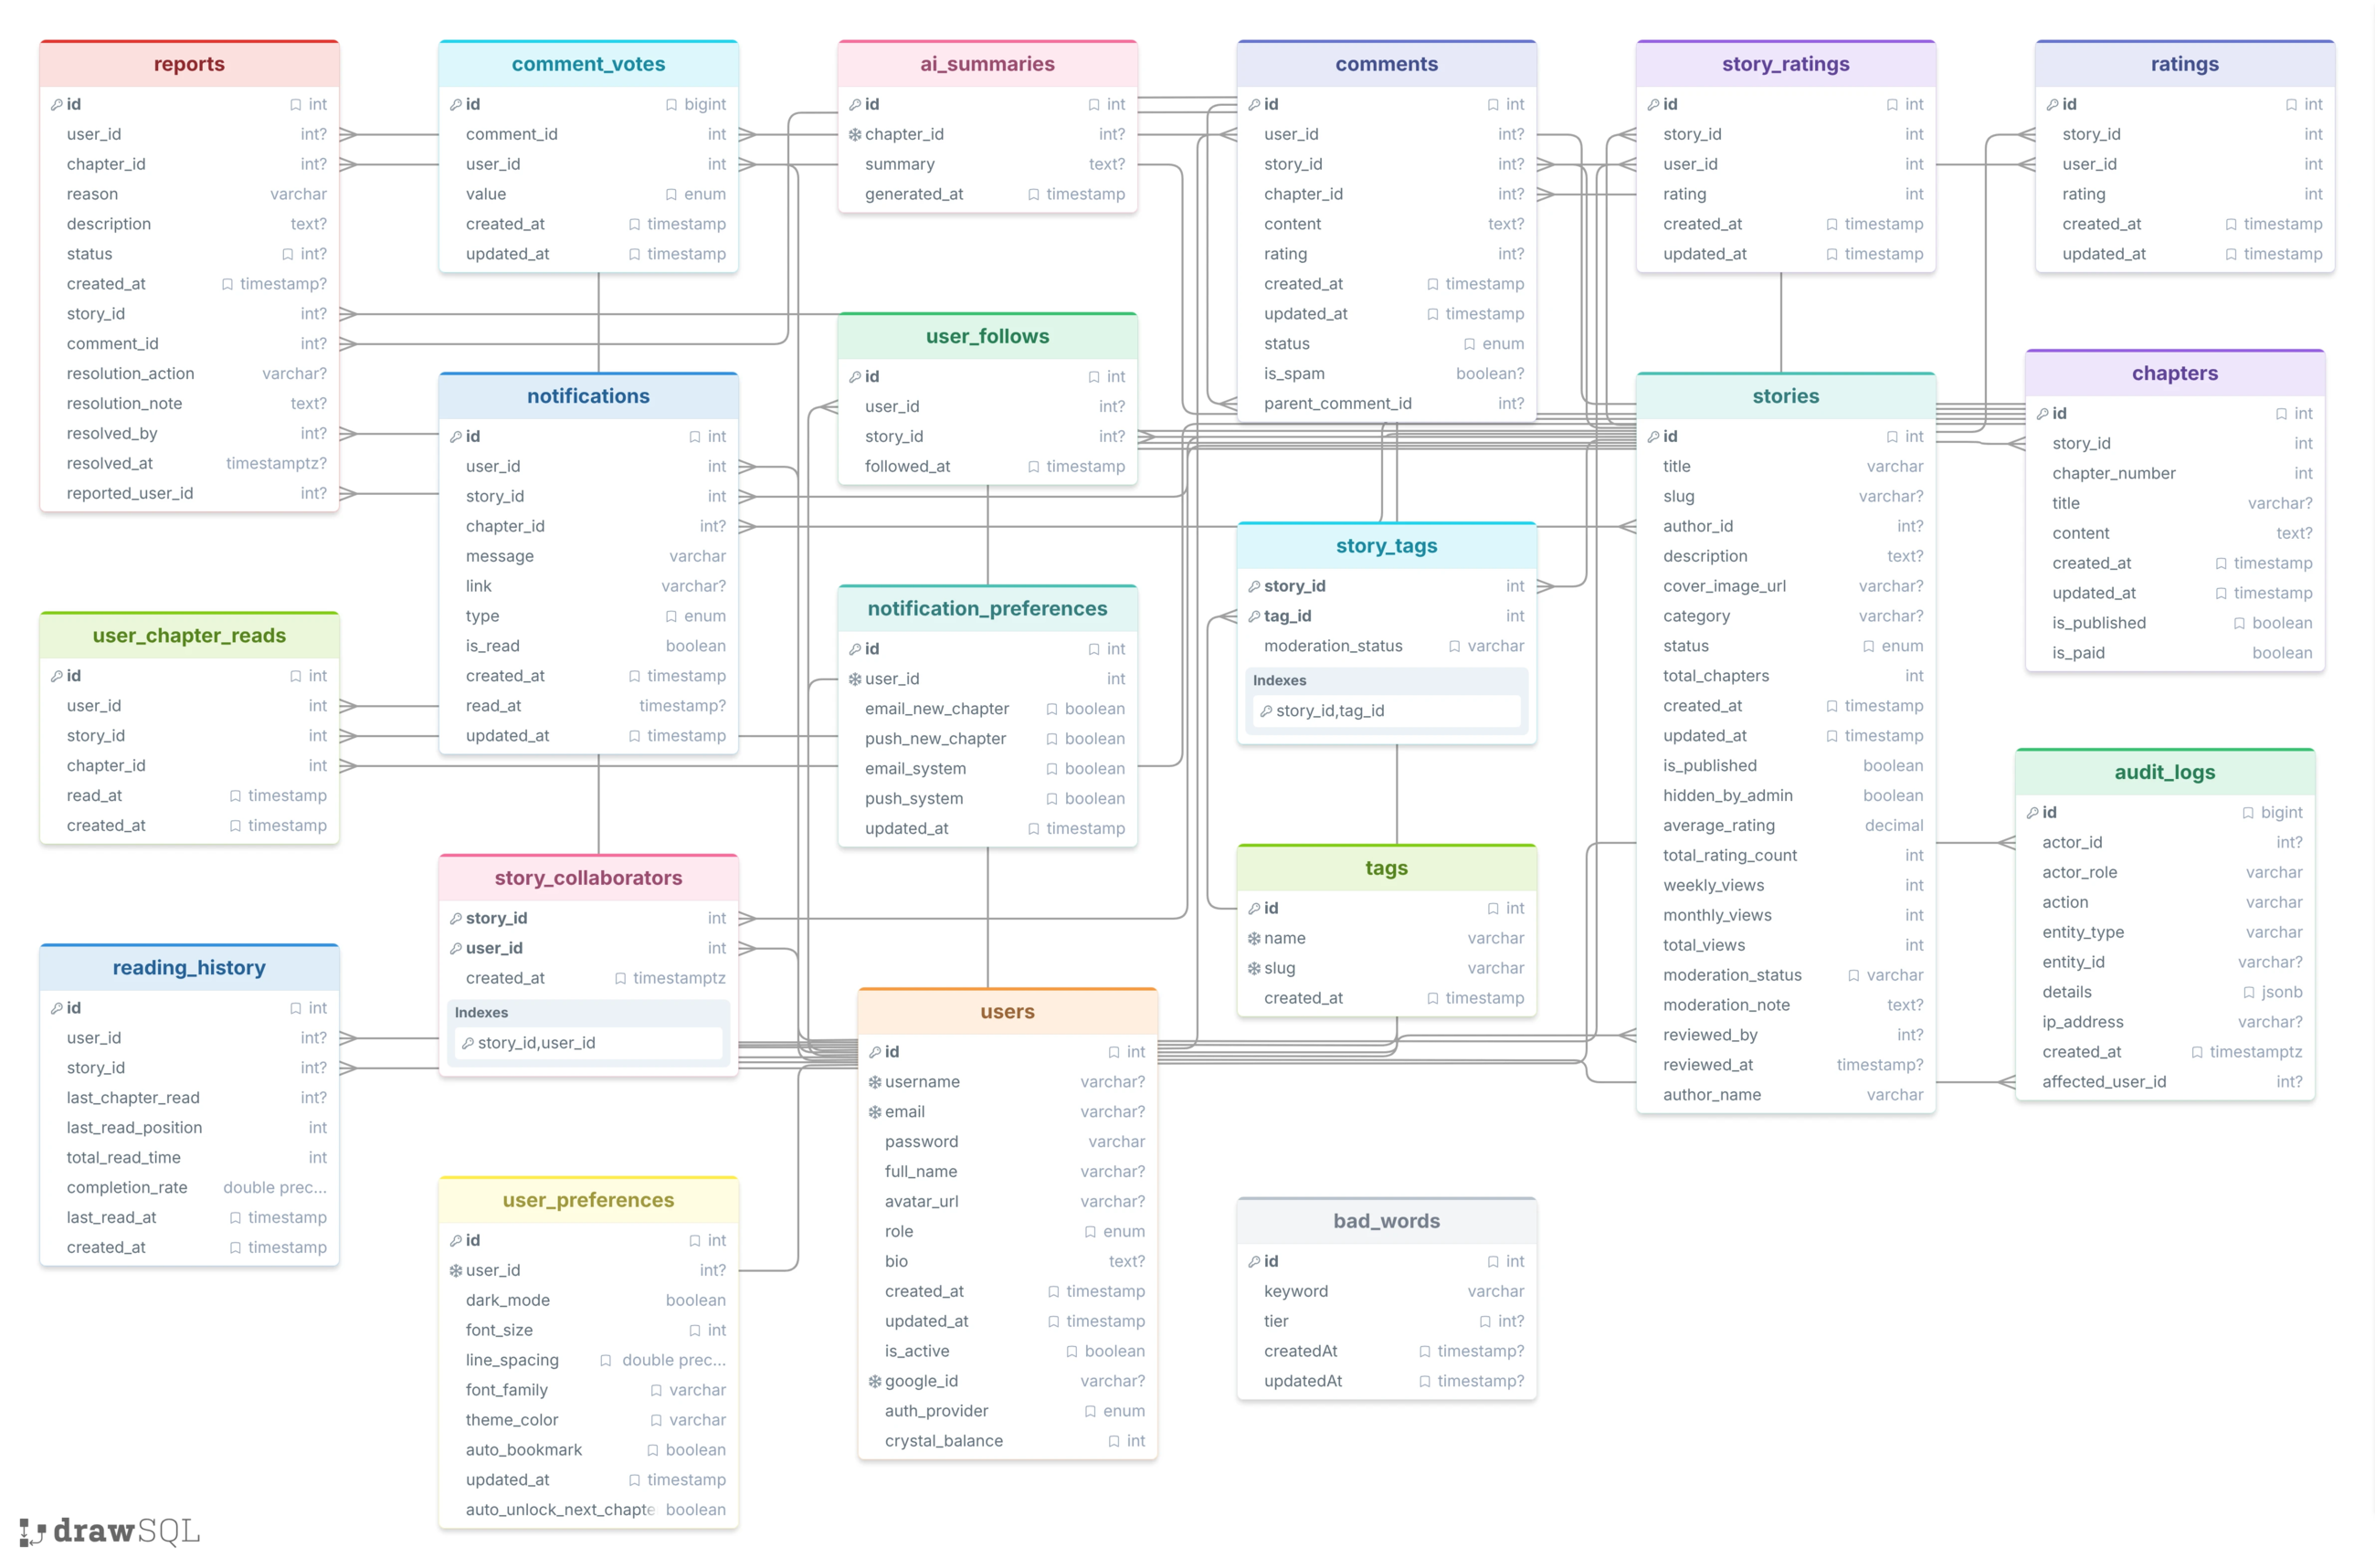
\includegraphics[width=\linewidth,height=0.85\textheight,keepaspectratio]{images/database-erd.png}
  \captionof{figure}{Lược đồ ERD của cơ sở dữ liệu CMC Truyện\label{fig:database-er}}
\end{center}
\vspace*{\fill}
\end{landscape}

Hình~\ref{fig:database-er} thể hiện các quan hệ chính của hệ thống. \CodePath{users}, \CodePath{stories} và \CodePath{chapters} là ba thực thể trung tâm; các bảng lịch sử đọc, theo dõi, đánh giá, bình luận và thông báo liên kết hành vi người dùng với nội dung. Nhóm bảng \CodePath{reports}, \CodePath{bad_words} và \CodePath{audit_logs} phục vụ kiểm duyệt và truy vết.


\ReportImage[1.0\textheight]
  {images/screenshots/db-folder-schema.png}
  {Cấu trúc script, migration và schema cơ sở dữ liệu}
  {fig:db-folder}
  {Chụp \CodePath{backend/scripts} và \CodePath{backend/src/scripts/migrations}; hiển thị tên file, không chụp chuỗi kết nối.}

\ReportImage[1.0\textheight]
  {images/screenshots/db-main-sql-code.png}
  {Đoạn SQL chính về bảng truyện, chương và ràng buộc}
  {fig:db-sql-code}
  {Chụp đoạn code thật trong \CodePath{schema.sql}, ưu tiên primary key, foreign key, CHECK, UNIQUE và index.}

\clearpage
\subsection{Connection pool, index và transaction}

Backend cấu hình PostgreSQL Pool với tối đa 20 connection, idle timeout 30 giây và connection timeout 5 giây. Môi trường production có thể dùng \CodePath{DATABASE_URL}; môi trường local có thể dùng các biến host/port/name/user/password. Index tập trung vào slug, danh sách truyện công khai, số chương, trạng thái bình luận, khóa ngoại và audit. API danh sách chương không trả trường content, qua đó giảm kích thước phản hồi.

Khi một nghiệp vụ có nhiều bước ghi dữ liệu, tất cả query từ \CodePath{BEGIN} đến \CodePath{COMMIT/ROLLBACK} phải dùng cùng client lấy từ \CodePath{pool.connect()}. Nếu trộn \CodePath{pool.query()} với client trong một transaction, các query có thể chạy trên connection khác và rollback không còn bảo đảm tính nguyên tử.
Nghiệp vụ mở khóa chương là ví dụ điển hình cho transaction nhiều bước. Model \CodePath{Wallet.unlockChapter} khóa bản ghi số dư của người dùng bằng \CodePath{FOR UPDATE}, kiểm tra bản ghi mở khóa hiện có và số dư trước khi ghi dữ liệu. Nếu bất kỳ bước nào thất bại, \CodePath{ROLLBACK} bảo đảm số dư, lịch sử giao dịch và quyền đọc không rơi vào trạng thái không nhất quán.



\section{Cấu hình và triển khai}

\subsection{Biến môi trường}

Các biến chính gồm URL frontend/backend, PostgreSQL, Redis, JWT, Google OAuth, Resend, Supabase và nhà cung cấp AI. File \CodePath{.env} không được commit. Frontend chỉ nhận biến public như \CodePath{VITE_API_URL}; service key, JWT secret và AI key phải ở backend.

\begin{table}[htbp]
\centering
\caption{Nhóm biến môi trường và nguyên tắc bảo mật}
\label{tab:environment-vars}
\begin{tabularx}{\textwidth}{|>{\bfseries\RaggedRight\arraybackslash}p{3.2cm}|X|X|}
\hline
\textbf{Nhóm} & \textbf{Ví dụ tên biến} & \textbf{Nguyên tắc} \\
\hline
Database & DATABASE\_URL, DB\_HOST, DB\_NAME & Chỉ backend; production ưu tiên secret manager. \\
\hline
Auth & JWT\_SECRET, GOOGLE\_CLIENT\_ID & Secret đủ mạnh; không dùng fallback production. \\
\hline
Queue & REDIS\_URL & API và worker dùng cùng instance; bật TLS nếu nhà cung cấp yêu cầu. \\
\hline
Email/Storage & RESEND\_API\_KEY, SUPABASE\_SERVICE\_KEY & Service key không xuất hiện trong bundle frontend/log. \\
\hline
AI & GROQ\_API\_KEY, GEMINI\_API\_KEY & Chỉ backend; đặt timeout, quota và theo dõi lỗi. \\
\hline
Frontend & VITE\_API\_URL & Có thể công khai; trỏ đúng tiền tố \CodePath{/\allowbreak{}api}. \\
\hline
\end{tabularx}
\end{table}

\subsection{Topology triển khai}

\CodePath{Render.yaml} khai báo hai service Node: web service chạy backend và worker chạy \CodePath{src/startWorker.js}. Frontend có \CodePath{vercel.json} rewrite mọi route SPA về \CodePath{index.html}. PostgreSQL và Redis không được khai báo trực tiếp trong file Render; chúng phải được cung cấp qua dịch vụ managed hoặc hạ tầng khác và cấu hình bằng environment.

\begin{table}[htbp]
\centering
\caption{Liên kết bàn giao và minh chứng triển khai}
\label{tab:delivery-links}
\begin{tabularx}{\textwidth}{|>{\bfseries\RaggedRight\arraybackslash}p{4.0cm}|X|}
\hline
\textbf{Hạng mục} & \textbf{Liên kết} \\
\hline
Website chạy thực tế & \OptionalURL{\WebsiteURL}{https://thanhnt2k.app/} \\
\hline
Kho source dùng để nộp & \OptionalURL{\SourceCodeURL}{https://github.com/suzynotsusie/cmc-truyen-temp} \\
\hline
\end{tabularx}
\end{table}

\clearpage

\section{Kiểm thử và kết quả xác minh}

\subsection{Chiến lược kiểm thử}

Dự án áp dụng chiến lược kiểm thử theo mô hình tháp (Testing Pyramid) với ba tầng chính: unit/integration test chiếm phần lớn (Jest cho backend, Vitest và Testing Library cho frontend), E2E test tự động bằng Playwright cho các luồng nghiệp vụ quan trọng, và kiểm thử thủ công bổ sung cho kịch bản khó tự động hóa. Toàn bộ dependency ngoài (database, Redis, Supabase, email) được mock trong bộ test mặc định để đảm bảo CI ổn định; kiểm thử với hạ tầng thật được lên kế hoạch trên môi trường staging riêng. Bảng~\ref{tab:test-tools} tóm tắt công cụ theo từng tầng.

\begin{table}[htbp]
\centering
\caption{Công cụ và phạm vi kiểm thử theo tầng}
\label{tab:test-tools}
\begin{tabularx}{\textwidth}{|>{\RaggedRight\arraybackslash}p{3.2cm}|>{\RaggedRight\arraybackslash}p{4.0cm}|X|}
\hline
\textbf{Tầng kiểm thử} & \textbf{Công cụ} & \textbf{Phạm vi} \\
\hline
Unit / Integration & Jest, Supertest & Backend: controller, service, middleware, RBAC, audit \\
\hline
Component / Unit & Vitest, Testing Library & Frontend: component, hook, route guard, UI behavior \\
\hline
End-to-End & Playwright & Luồng đăng nhập, tìm kiếm và đọc truyện \\
\hline
Performance & Jest (budget test) & Parse 1.000 chương trong ngân sách thời gian định nghĩa \\
\hline
Thủ công & Trình duyệt, DevTools & Responsive, edge case UX, luồng phân quyền phức tạp \\
\hline
\end{tabularx}
\end{table}

\subsection{Kết quả tổng hợp}

Bộ test mặc định và build frontend được chạy trực tiếp trên workspace dự án. Kết quả được ghi ở Bảng~\ref{tab:test-results}; đây là số liệu của lần chạy thực tế, không phải con số giả định.

\begin{table}[H]
\centering
\caption{Kết quả kiểm thử và build đã thực chạy}
\label{tab:test-results}
\begin{tabularx}{\textwidth}{|>{\RaggedRight\arraybackslash}p{4.0cm}|>{\centering\arraybackslash}p{2.5cm}|X|}
\hline
\textbf{Hạng mục} & \textbf{Kết quả} & \textbf{Ghi chú quan sát} \\
\hline
Backend (Jest) & 121/121 pass & 21 test suite pass; có log Redis \CodePath{ECONNREFUSED} và Jest force-exit do \CodePath{BullMQ} queue chưa đóng sau test. \\
\hline
Frontend (Vitest) & 36/36 pass & 11 test file pass; có cảnh báo tùy chọn \CodePath{esbuild}/\CodePath{oxc} deprecated từ toolchain. \\
\hline
Tổng test mặc định & 157/157 pass & Lệnh root test hoàn thành exit code 0. \\
\hline
Frontend production build & Thành công & 209 module transformed; build trong 2,13 giây; cảnh báo dynamic import cho \CodePath{mockStories.js}. \\
\hline
Bundle JavaScript & 641,96 kB & Gzip 192,47 kB; Vite cảnh báo chunk lớn hơn 500 kB. \\
\hline
E2E Playwright & 6/6 pass & 100\% pass (6 kịch bản: login reader, login sai, mất mạng, login admin, tìm kiếm, đọc chương). \\
\hline
Performance (parse 1.000 chương) & Đạt ngân sách & Service parse tệp hoàn thành dưới ngưỡng thời gian định nghĩa trong \CodePath{storyFileImportService.\allowbreak{}performance.\allowbreak{}test.js}. \\
\hline
\end{tabularx}
\end{table}

Các bài kiểm thử đều đã vượt qua thành công, chứng minh các vùng logic cốt lõi đã được bảo vệ đầy đủ: từ health, auth, RBAC, audit, OTP, đến import file, ranking, kiểm duyệt, báo cáo và luồng xử lý truyện. Lỗi kết nối Redis \CodePath{ECONNREFUSED} xuất hiện trong log là bình thường khi chạy ở môi trường local không có sẵn service Redis. Về việc Jest bị force-exit, nguyên nhân xuất phát từ việc hàng đợi \CodePath{BullMQ} chưa được đóng đúng cách trong \CodePath{afterAll}. Để khắc phục triệt để, chúng ta cần bổ sung logic teardown nhằm giải phóng kết nối, đồng thời tích hợp \CodePath{ioredis-mock} để cô lập hoàn toàn các unit test. Cuối cùng, kích thước bundle JavaScript hiện đạt 641,96~kB, vượt quá giới hạn khuyến nghị 500~kB của Vite. Giải pháp cần triển khai là áp dụng route-level lazy loading kết hợp chia nhỏ vendor chunk, sau đó đo đạc lại để kiểm chứng.
\clearpage

\subsection{Nhóm 1: Xác thực người dùng}

Kết quả kiểm thử tự động cho luồng xác thực người dùng (đăng nhập, đăng ký, quên mật khẩu và xác thực OTP) được tổng hợp tại Bảng~\ref{tab:tc-auth}. Quá trình kiểm thử bao gồm 18 kịch bản, được thực thi qua các test suite: \CodePath{authController.login.test.js}, \CodePath{authController.account.test.js} và \CodePath{otpService.test.js}, nhằm đảm bảo tính bảo mật và trải nghiệm xuyên suốt của hệ thống.

\begingroup
\footnotesize
\begin{longtable}{|>{\centering\arraybackslash}p{0.5cm}|>{\RaggedRight\arraybackslash}p{2.0cm}|>{\RaggedRight\arraybackslash}p{3.5cm}|>{\RaggedRight\arraybackslash}p{2.2cm}|>{\RaggedRight\arraybackslash}p{2.2cm}|>{\RaggedRight\arraybackslash}p{3.1cm}|}
\caption{Test case nhóm xác thực người dùng}\label{tab:tc-auth}\\
\hline
\textbf{STT} & \textbf{Test Case} & \textbf{Input} & \textbf{Output} & \textbf{Kết quả mong muốn} & \textbf{Kết quả thực tế} \\
\hline
\endfirsthead
\hline
\textbf{STT} & \textbf{Test Case} & \textbf{Input} & \textbf{Output} & \textbf{Kết quả mong muốn} & \textbf{Kết quả thực tế} \\
\hline
\endhead
\hline
\multicolumn{6}{|r|}{\emph{Còn tiếp ở trang sau}}\\
\hline
\endfoot
\hline
\endlastfoot
1 & Đăng nhập đúng tài khoản & Email \texttt{reader\allowbreak{}@\allowbreak{}example.\allowbreak{}com}, password \texttt{Password1!} & HTTP \texttt{200}, JWT và user & Đăng nhập thành công; response không chứa password & HTTP \texttt{200}, có token, password đã bị loại bỏ (\textbf{Đạt}) \\
\hline
2 & Đúng email, sai mật khẩu & Email hợp lệ, password \texttt{WrongPassword1!} & HTTP \texttt{401}, thông báo tiếng Việt & Không cấp token & HTTP \texttt{401}, UI hiển thị thông báo tiếng Việt (\textbf{Đạt}) \\
\hline
3 & Sai email, đúng mật khẩu của tài khoản khác & Email \texttt{unknown\allowbreak{}@\allowbreak{}example.\allowbreak{}com}, password hợp lệ & HTTP \texttt{401}, cùng thông báo lỗi & Không đăng nhập và không tiết lộ email tồn tại hay không & HTTP \texttt{401}, cùng thông báo tiếng Việt (\textbf{Đạt}) \\
\hline
4 & Email đăng nhập sai định dạng & \texttt{reader-at-\allowbreak{}example.\allowbreak{}com} & HTTP \texttt{400}, lỗi định dạng & Chặn trước khi truy vấn database & HTTP \texttt{400}, lỗi hiển thị bằng tiếng Việt (\textbf{Đạt}) \\
\hline
5 & Email dùng ký tự Unicode full-width & Chuỗi email toàn ký tự full-width & HTTP \texttt{400}, dữ liệu không hợp lệ & Không chấp nhận định dạng ký tự sai & HTTP \texttt{400}, không truy vấn user (\textbf{Đạt}) \\
\hline
6 & Database lỗi khi đăng nhập & Credentials hợp lệ; DB không khả dụng & HTTP \texttt{500}, thông báo chung & Không cấp token và không lộ lỗi nội bộ & HTTP \texttt{500}, thông báo chung bằng tiếng Việt (\textbf{Đạt}) \\
\hline
7 & Đăng ký hợp lệ & Username \texttt{Reader\_01}, email hợp lệ, password mạnh & HTTP \texttt{201}, token và role \texttt{User} & Tạo tài khoản, hash password, không trả hash & Role \texttt{User}, response không có password (\textbf{Đạt}) \\
\hline
8 & Username đã tồn tại & Username trùng tài khoản hiện có & HTTP \texttt{409} & Không kiểm tra/tạo tiếp bằng email & HTTP \texttt{409}, không gọi tạo user (\textbf{Đạt}) \\
\hline
9 & Email đã tồn tại & Username mới, email trùng & HTTP \texttt{409} & Không tạo tài khoản trùng & HTTP \texttt{409}, không gọi tạo user (\textbf{Đạt}) \\
\hline
10 & Username sai định dạng & Username có dấu hoặc khoảng trắng & HTTP \texttt{400} & Chỉ nhận chữ không dấu, số, \texttt{\_}, \texttt{-} & HTTP \texttt{400}, thông báo tiếng Việt (\textbf{Đạt}) \\
\hline
11 & Mật khẩu đăng ký yếu & \texttt{password} (thiếu chữ hoa, số, ký tự đặc biệt) & HTTP \texttt{400}, thông báo tiêu chí & Yêu cầu tối thiểu 8 ký tự, chữ hoa, số và ký tự đặc biệt & HTTP \texttt{400}, không tạo user (\textbf{Đạt}) \\
\hline
12 & Chèn role qua request đăng ký & Payload có thêm \texttt{role: Admin} và \texttt{is\_\allowbreak{}active: false} & User tạo với role \texttt{User} & Chống mass assignment & Field lạ bị loại bỏ, role vẫn là \texttt{User} (\textbf{Đạt}) \\
\hline
13 & Quên mật khẩu với email tồn tại/không tồn tại & Hai email có trạng thái khác nhau & Cùng HTTP \texttt{200} và cùng message & Chống dò tìm email tài khoản & Hai response giống nhau (\textbf{Đạt}) \\
\hline
14 & OTP sai hoặc hết hạn & OTP \texttt{000000} không hợp lệ & HTTP \texttt{400} & Không cho reset password & HTTP \texttt{400}, không cập nhật password (\textbf{Đạt}) \\
\hline
15 & Reset khi chưa xác thực OTP & Password mới hợp lệ nhưng OTP chưa verified & HTTP \texttt{403} & Bắt buộc xác thực OTP trước & HTTP \texttt{403}, không cập nhật password (\textbf{Đạt}) \\
\hline
16 & Reset password thành công & OTP verified; password mạnh và xác nhận khớp & HTTP \texttt{200} & Hash password mới và xóa OTP đã dùng & Password được cập nhật, OTP keys được xóa (\textbf{Đạt}) \\
\hline
17 & Gửi form login hai lần (double-click) & Double-click nút đăng nhập khi request đang xử lý & Chỉ một request; nút bị disabled & Không tạo request đăng nhập trùng & Hàm login chỉ được gọi một lần (\textbf{Đạt}) \\
\hline
18 & Mất mạng khi đăng nhập & API login bị ngắt kết nối & UI giữ nguyên \texttt{/\allowbreak{}login} và hiện lỗi & Cho phép người dùng thử lại, không crash & Alert lỗi hiển thị, không chuyển trang (\textbf{Đạt}) \\
\hline
\end{longtable}
\endgroup

\clearpage

\subsection{Nhóm 2: Upload truyện và kiểm duyệt}

Quy trình đăng tải truyện và các bước kiểm duyệt được đánh giá qua 21 kịch bản kiểm thử tự động (Bảng~\ref{tab:tc-upload}). Quá trình này xác minh các ràng buộc về quyền sở hữu, giới hạn kích thước tệp tải lên (tối đa 25~MB) và luồng công việc xét duyệt của Moderator. Các test suite đảm nhiệm bao gồm: \CodePath{uploadStoryFile.test.js}, \CodePath{chapterController.upload.test.js}, \CodePath{storyWorkflow.test.js} và \CodePath{moderatorController.test.js}.

\begingroup
\footnotesize
\begin{longtable}{|>{\centering\arraybackslash}p{0.5cm}|>{\RaggedRight\arraybackslash}p{2.0cm}|>{\RaggedRight\arraybackslash}p{3.5cm}|>{\RaggedRight\arraybackslash}p{2.2cm}|>{\RaggedRight\arraybackslash}p{2.2cm}|>{\RaggedRight\arraybackslash}p{3.1cm}|}
\caption{Test case nhóm upload truyện và kiểm duyệt}\label{tab:tc-upload}\\
\hline
\textbf{STT} & \textbf{Test Case} & \textbf{Input} & \textbf{Output} & \textbf{Kết quả mong muốn} & \textbf{Kết quả thực tế} \\
\hline
\endfirsthead
\hline
\textbf{STT} & \textbf{Test Case} & \textbf{Input} & \textbf{Output} & \textbf{Kết quả mong muốn} & \textbf{Kết quả thực tế} \\
\hline
\endhead
\hline
\multicolumn{6}{|r|}{\emph{Còn tiếp ở trang sau}}\\
\hline
\endfoot
\hline
\endlastfoot
1 & Upload TXT UTF-8 vào truyện đã duyệt & Uploader là chủ sở hữu; \texttt{truyen.txt} UTF-8; truyện approved & HTTP \texttt{201},\newline\texttt{imported\_\allowbreak{}count: 1} & Tạo đúng chương và số chương kế tiếp & Tạo 1 chương, \texttt{next\_\allowbreak{}chapter\_\allowbreak{}number: 2} (\textbf{Đạt}) \\
\hline
2 & Upload nội dung UTF-16 LE tiếng Việt & TXT có BOM UTF-16 LE & HTTP \texttt{200} khi preview & Không lỗi font hoặc mất dấu & Tiêu đề/nội dung tiếng Việt giữ nguyên (\textbf{Đạt}) \\
\hline
3 & Không chọn file & Request không có field \texttt{file} & HTTP \texttt{400} & Không tạo chương, báo thiếu file & HTTP \texttt{400}, batch insert không được gọi (\textbf{Đạt}) \\
\hline
4 & File không có nội dung đọc được & TXT chỉ chứa byte NUL & HTTP \texttt{400},\newline\texttt{success: false} & Không import dữ liệu rác & HTTP \texttt{400}, không tạo chương (\textbf{Đạt}) \\
\hline
5 & Sai đuôi file & \texttt{truyen.exe} & HTTP \texttt{400} & Chỉ chấp nhận \texttt{.txt}, \texttt{.md}, \texttt{.epub} & Middleware từ chối file (\textbf{Đạt}) \\
\hline
6 & Đuôi đúng nhưng MIME sai & \texttt{truyen.txt}, MIME \texttt{image/\allowbreak{}png} & HTTP \texttt{400} & Kiểm tra cả extension và MIME type & Middleware trả lỗi định dạng (\textbf{Đạt}) \\
\hline
7 & File vượt kích thước 25~MB & TXT lớn hơn 25~MB & HTTP \texttt{400},\newline\texttt{LIMIT\_\allowbreak{}FILE\_\allowbreak{}SIZE} & Chặn file quá giới hạn & Nhận đúng mã\newline\texttt{LIMIT\_\allowbreak{}FILE\_\allowbreak{}SIZE} (\textbf{Đạt}) \\
\hline
8 & Chưa đăng nhập khi import & Không có \texttt{req.user} & HTTP \texttt{401} & Yêu cầu xác thực & HTTP \texttt{401}, không truy vấn truyện (\textbf{Đạt}) \\
\hline
9 & Uploader không sở hữu truyện & User \texttt{99} import vào truyện của user \texttt{7} & HTTP \texttt{403} & Chỉ owner/\allowbreak{}collaborator/\allowbreak{}Admin được thao tác & HTTP \texttt{403}, không tạo chương (\textbf{Đạt}) \\
\hline
10 & Import khi truyện chưa duyệt & Truyện \texttt{pending}, chưa publish & HTTP \texttt{409} & Chỉ import sau khi Moderator duyệt & HTTP \texttt{409}, không tạo chương (\textbf{Đạt}) \\
\hline
11 & Database lỗi khi import & File hợp lệ; DB không khả dụng & HTTP \texttt{500},\newline\texttt{success: false} & Không trả số chương thành công giả & HTTP \texttt{500}, không trả success (\textbf{Đạt}) \\
\hline
12 & Tạo truyện mới & Metadata hợp lệ từ Uploader & HTTP \texttt{201}; truyện chờ duyệt & Lưu uploader và tên tác giả riêng biệt & \texttt{author\_\allowbreak{}id} và \texttt{author\_\allowbreak{}name} lưu đúng (\textbf{Đạt}) \\
\hline
13 & Thêm chương trước khi truyện được duyệt & Truyện \texttt{pending} & HTTP \texttt{409} & Không cho thêm chương & HTTP \texttt{409}, model tạo chương không được gọi (\textbf{Đạt}) \\
\hline
14 & Số chương bị trùng & Chapter number đã tồn tại & HTTP \texttt{409},\newline\texttt{CHAPTER\_\allowbreak{}NUMBER\_\allowbreak{}EXISTS} & Không trả lỗi máy chủ chung chung & HTTP \texttt{409}, đúng mã nghiệp vụ (\textbf{Đạt}) \\
\hline
15 & Uploader tự publish truyện & Uploader gọi toggle visibility & HTTP \texttt{403} & Xuất bản phải qua Moderator/\allowbreak{}Admin & HTTP \texttt{403}, không cập nhật truyện (\textbf{Đạt}) \\
\hline
16 & Preview file truyện & TXT có heading chương & HTTP \texttt{200}, danh sách preview & Preview không tạo dữ liệu chương & Có preview, \texttt{Chapter.\allowbreak{}createChapter} không được gọi (\textbf{Đạt}) \\
\hline
17 & Moderator duyệt truyện pending & Story đang trong moderation queue & HTTP \texttt{200} & Chuyển trạng thái đúng và publish & Truyện được duyệt theo workflow (\textbf{Đạt}) \\
\hline
18 & Moderator yêu cầu sửa có lý do & Action request changes và reason hợp lệ & HTTP thành công, có notification & Lưu lý do và thông báo Uploader & Trạng thái và notification được cập nhật (\textbf{Đạt}) \\
\hline
19 & Moderator yêu cầu sửa thiếu lý do & Action request changes, reason rỗng & HTTP \texttt{400} & Bắt buộc có lý do & HTTP \texttt{400}, không cập nhật truyện (\textbf{Đạt}) \\
\hline
20 & Moderator lọc danh sách theo tiêu chí & Status/\allowbreak{}search/\allowbreak{}page/\allowbreak{}limit & Danh sách và global status counts & Lọc đúng; count phản ánh toàn hệ thống & Kết quả lọc và counts đúng (\textbf{Đạt}) \\
\hline
21 & Xử lý report avatar & Report avatar gắn với user bị báo cáo & HTTP thành công & Cập nhật đúng boolean/status, không nhầm enum & Tham số cập nhật tách biệt đúng (\textbf{Đạt}) \\
\hline
\end{longtable}
\endgroup

\clearpage

\subsection{Nhóm 3: Chức năng người dùng}

Các tính năng tương tác của người dùng như tìm kiếm, theo dõi truyện, bình luận, đánh giá, báo cáo vi phạm, tải ảnh đại diện và mở khóa chương bằng Tinh thạch được kiểm chứng thông qua 29 kịch bản (Bảng~\ref{tab:tc-user}). Việc kiểm thử được thực hiện qua các test suite: \CodePath{socialInteractions.test.js}, \CodePath{storyDiscoveryRating.test.js}, \CodePath{reportController.test.js}, \CodePath{chapterUnlock.test.js} và \CodePath{uploadCover.test.js}.

\begingroup
\footnotesize
\begin{longtable}{|>{\centering\arraybackslash}p{0.5cm}|>{\RaggedRight\arraybackslash}p{2.0cm}|>{\RaggedRight\arraybackslash}p{3.5cm}|>{\RaggedRight\arraybackslash}p{2.2cm}|>{\RaggedRight\arraybackslash}p{2.2cm}|>{\RaggedRight\arraybackslash}p{3.1cm}|}
\caption{Test case nhóm chức năng người dùng}\label{tab:tc-user}\\
\hline
\textbf{STT} & \textbf{Test Case} & \textbf{Input} & \textbf{Output} & \textbf{Kết quả mong muốn} & \textbf{Kết quả thực tế} \\
\hline
\endfirsthead
\hline
\textbf{STT} & \textbf{Test Case} & \textbf{Input} & \textbf{Output} & \textbf{Kết quả mong muốn} & \textbf{Kết quả thực tế} \\
\hline
\endhead
\hline
\multicolumn{6}{|r|}{\emph{Còn tiếp ở trang sau}}\\
\hline
\endfoot
\hline
\endlastfoot
1 & Upload avatar JPG/\allowbreak{}PNG/\allowbreak{}WebP hợp lệ & File nhỏ hơn hoặc bằng 5~MB, MIME ảnh & HTTP \texttt{200} qua middleware & Chấp nhận các ảnh hợp lệ & Cả JPG, PNG, WebP đều được nhận (\textbf{Đạt}) \\
\hline
2 & Upload file script giả avatar & \texttt{..\allowbreak{}/\allowbreak{}attack.svg}, MIME \texttt{text/\allowbreak{}html} & HTTP \texttt{400} & Không nhận nội dung không phải ảnh & Middleware từ chối (\textbf{Đạt}) \\
\hline
3 & Avatar vượt 5~MB & PNG lớn hơn 5~MB & HTTP \texttt{400},\newline\texttt{LIMIT\_\allowbreak{}FILE\_\allowbreak{}SIZE} & Chặn file quá lớn & Nhận đúng mã giới hạn (\textbf{Đạt}) \\
\hline
4 & Tìm kiếm kết hợp & Query có dấu/ký tự đặc biệt, category, tag, page & HTTP \texttt{200}, stories và pagination & Truyền đúng bộ lọc, không crash & Model nhận đúng tham số, HTTP \texttt{200} (\textbf{Đạt}) \\
\hline
5 & Tìm kiếm không có kết quả & Từ khóa không tồn tại & HTTP \texttt{200},\newline\texttt{stories: []} & Danh sách rỗng không phải lỗi & HTTP \texttt{200}, mảng rỗng (\textbf{Đạt}) \\
\hline
6 & Guest xem truyện nháp & Slug của truyện chưa publish & HTTP \texttt{404} & Không lộ nội dung chưa duyệt & HTTP \texttt{404} (\textbf{Đạt}) \\
\hline
7 & Guest kiểm tra trạng thái follow & Không có user/token & HTTP \texttt{200},\newline\texttt{following: false} & Endpoint optional auth không trả \texttt{401} & HTTP \texttt{200}, \texttt{false} (\textbf{Đạt}) \\
\hline
8 & Follow/unfollow lặp lại & Gọi follow hai lần, unfollow hai lần & Các request thành công/idempotent & Không gây lỗi hoặc dữ liệu trùng & Controller xử lý các lần gọi ổn định (\textbf{Đạt}) \\
\hline
9 & Follow với story ID sai & ID \texttt{0}, \texttt{-1}, \texttt{abc} & HTTP \texttt{400} & Chỉ nhận ID nguyên dương & Cả ba trường hợp đều bị từ chối (\textbf{Đạt}) \\
\hline
10 & Follow API thất bại, UI tự động rollback & UI cập nhật trước (optimistic); API reject & UI rollback trạng thái & Không để trạng thái giả trên giao diện & Nút follow quay lại trạng thái trước (\textbf{Đạt}) \\
\hline
11 & Bình luận rỗng hoặc quá dài & Khoảng trắng hoặc hơn 2.000 ký tự & HTTP \texttt{400} & Không tạo bình luận sai & HTTP \texttt{400}, model create không được gọi (\textbf{Đạt}) \\
\hline
12 & Reply sang thread khác & Parent thuộc story/\allowbreak{}chapter khác & HTTP \texttt{400} & Không gắn reply sai thread & HTTP \texttt{400}, không tạo comment (\textbf{Đạt}) \\
\hline
13 & User xóa bình luận của người khác & User thường không phải owner & HTTP \texttt{403} & Bảo vệ quyền sở hữu comment & HTTP \texttt{403}, không xóa (\textbf{Đạt}) \\
\hline
14 & Admin xóa bình luận bất kỳ & Admin xóa comment của user khác & HTTP \texttt{200} & Admin được phép moderation & Comment được xóa (\textbf{Đạt}) \\
\hline
15 & Vote sai giá trị & Vote \texttt{0}, \texttt{2}, \texttt{-2} & HTTP \texttt{400} & Chỉ nhận \texttt{1} hoặc \texttt{-1} & Cả ba giá trị bị từ chối (\textbf{Đạt}) \\
\hline
16 & Rating ngoài khoảng hợp lệ & Rating \texttt{0}, \texttt{6}, \texttt{1.5}, \texttt{"five"} & HTTP \texttt{400} & Chỉ nhận số nguyên 1--5 & Không gọi upsert rating (\textbf{Đạt}) \\
\hline
17 & Thêm/cập nhật rating hợp lệ & Rating \texttt{5} của user đăng nhập & HTTP \texttt{200}, summary mới & Upsert rating của đúng user & Model nhận story ID, user ID và rating đúng (\textbf{Đạt}) \\
\hline
18 & Xóa rating của chính user & User xóa rating của mình & HTTP \texttt{200}, summary mới & Không xóa rating của user khác & Model được gọi với đúng user hiện tại (\textbf{Đạt}) \\
\hline
19 & Tạo report hợp lệ & User, target story, reason, description & HTTP \texttt{201} & Tạo report đúng target & Insert đúng dữ liệu (\textbf{Đạt}) \\
\hline
20 & Spam report vượt rate limit & Đã gửi đủ giới hạn trong một giờ & HTTP \texttt{429} & Chặn spam trước khi insert & HTTP \texttt{429}, không insert report (\textbf{Đạt}) \\
\hline
21 & Report avatar từ comment & Comment ID có tác giả & Report gắn\newline\texttt{reported\_\allowbreak{}user\_\allowbreak{}id} & Moderator biết đúng user bị báo cáo & User ID được lấy từ tác giả comment (\textbf{Đạt}) \\
\hline
22 & Cập nhật report không tồn tại & Report ID không có trong DB & HTTP \texttt{404} & Không tạo trạng thái giả & HTTP \texttt{404} (\textbf{Đạt}) \\
\hline
23 & Hành động report sai loại target & Dùng chapter action cho comment report & HTTP \texttt{400} & Chặn action không tương thích & HTTP \texttt{400}, không cập nhật target (\textbf{Đạt}) \\
\hline
24 & Mở khóa chương miễn phí & Chapter \texttt{is\_\allowbreak{}paid: false} & HTTP \texttt{409}, không trừ tiền & Không gọi giao dịch ví & Wallet không được gọi (\textbf{Đạt}) \\
\hline
25 & Mở khóa chương trả phí & Chapter khóa; số dư đủ & HTTP \texttt{200},\newline\texttt{CHAPTER\_\allowbreak{}UNLOCKED} & Trừ đúng \CodePath{UNLOCK_COST} và trả số dư mới & Chương được mở, số dư giảm đúng chi phí cấu hình (\textbf{Đạt}) \\
\hline
26 & Mở khóa lại hoặc request đồng thời & Wallet báo\newline\texttt{already\_\allowbreak{}unlocked: true} & HTTP \texttt{200}, cost \texttt{0} & Không trừ tiền lần hai & \texttt{CHAPTER\_\allowbreak{}ALREADY\_\allowbreak{}UNLOCKED}, cost \texttt{0} (\textbf{Đạt}) \\
\hline
27 & Số dư không đủ khi mở khóa & Balance nhỏ hơn \CodePath{UNLOCK_COST} & HTTP \texttt{409},\newline\texttt{INS\allowbreak{}UFFICI\allowbreak{}ENT\_\allowbreak{}CRYSTALS} & Không mở khóa; trả số dư hiện tại & API trả \texttt{409}, số dư không thay đổi (\textbf{Đạt}) \\
\hline
28 & Database lỗi khi mở khóa & DB error chứa dữ liệu nội bộ & HTTP \texttt{500}, thông báo chung & Không lộ chi tiết database & UI chỉ hiển thị thông báo chung tiếng Việt (\textbf{Đạt}) \\
\hline
\end{longtable}
\endgroup

\clearpage

\subsection{Kiểm thử thủ công bổ sung}

Đối với các nghiệp vụ phức tạp liên quan đến trải nghiệm tương tác giao diện (UI/UX), khả năng hiển thị tương thích đa thiết bị và sự tích hợp với các dịch vụ bên ngoài trong điều kiện thực tế, hệ thống được xác minh bổ sung thông qua phương pháp kiểm thử thủ công. Kết quả đánh giá cho 10 kịch bản đặc thù này được tổng hợp chi tiết tại Bảng~\ref{tab:manual-tests}, qua đó khẳng định hệ thống đáp ứng đầy đủ các yêu cầu đã đặt ra.

\begingroup
\footnotesize
\begin{longtable}{|>{\centering\arraybackslash}p{0.7cm}|>{\RaggedRight\arraybackslash}p{2.0cm}|>{\RaggedRight\arraybackslash}p{3.5cm}|>{\RaggedRight\arraybackslash}p{2.0cm}|>{\RaggedRight\arraybackslash}p{2.2cm}|>{\RaggedRight\arraybackslash}p{3.1cm}|}
\caption{Kịch bản kiểm thử thủ công bổ sung}\label{tab:manual-tests}\\
\hline
\textbf{STT} & \textbf{Test Case} & \textbf{Input} & \textbf{Output} & \textbf{Kết quả mong muốn} & \textbf{Kết quả thực tế} \\
\hline
\endfirsthead
\hline
\textbf{STT} & \textbf{Test Case} & \textbf{Input} & \textbf{Output} & \textbf{Kết quả mong muốn} & \textbf{Kết quả thực tế} \\
\hline
\endhead
\hline
\multicolumn{6}{|r|}{\emph{Còn tiếp ở trang sau}}\\
\hline
\endfoot
\hline
\endlastfoot
MT01 & Xem và đọc truyện public không cần đăng nhập & Guest; có truyện approved; từ khóa tìm kiếm & Trang reader và chi tiết hiển thị bình thường & Không yêu cầu login; URL đúng slug/\allowbreak{}chương & Hiển thị trang reader đầy đủ, URL chứa slug chuẩn (\textbf{Đạt}) \\
\hline
MT02 & Follow truyện và kiểm tra tính nhất quán & User đăng nhập; follow, tải lại, xem danh sách theo dõi & Trạng thái follow đồng bộ DB & Nhất quán với DB; lỗi mạng có rollback & Trạng thái follow/unfollow đồng bộ ngay sau khi tải lại (\textbf{Đạt}) \\
\hline
MT03 & Ghi nhận lịch sử đọc đúng user & User đọc nhiều chương; đọc, cuộn, thoát và mở lịch sử & Lịch sử hiển thị đúng & Trở về đúng truyện/chương; không ghi nhầm user & Lịch sử được lưu đúng tài khoản và vị trí chương đã đọc (\textbf{Đạt}) \\
\hline
MT04 & Uploader không thể thêm chương/publish khi pending & Uploader; truyện pending, chưa duyệt & HTTP \texttt{409}/\texttt{403}, thông báo rõ ràng & Bị chặn với thông báo đúng; không đổi DB & Uploader nhận lỗi HTTP \texttt{409}/\texttt{403} trên cả UI và API (\textbf{Đạt}) \\
\hline
MT05 & Moderator duyệt có/không có lý do & Moderator; truyện pending; lần~1 không nhập lý do, lần~2 nhập lý do & Lần~1: HTTP \texttt{400}; Lần~2: HTTP \texttt{200} & Lần đầu bị validate; lần sau cập nhật trạng thái, notify và audit & Bị chặn khi gửi lý do trống; duyệt thành công khi điền đủ lý do (\textbf{Đạt}) \\
\hline
MT06 & Rate limit khi gửi report nhiều lần & User; gửi report lặp trong 1 giờ & Report đầu: HTTP \texttt{201}; lần sau: HTTP \texttt{429} & Report đầu hợp lệ; request lặp bị hạn chế & API phản hồi HTTP \texttt{429} sau khi gửi report dồn dập (\textbf{Đạt}) \\
\hline
MT07 & Admin thay đổi role/\allowbreak{}status người dùng & Admin đăng nhập; chọn user, đổi role/\allowbreak{}status & UI cập nhật; audit log ghi nhận & UI cập nhật; audit không chứa password/token & Quyền user thay đổi ngay lập tức, audit log ghi nhận đầy đủ (\textbf{Đạt}) \\
\hline
MT08 & Token hết hạn không gây vòng lặp redirect & Token hết hạn; truy cập trang account/\allowbreak{}admin & HTTP \texttt{401}; redirect về \texttt{/\allowbreak{}login} & API trả \texttt{401}; frontend xóa phiên, không lặp vô hạn & API trả \texttt{401}; frontend xóa session và redirect về \texttt{/login} (\textbf{Đạt}) \\
\hline
MT09 & Responsive UI trên mobile và desktop & Viewport 375px và desktop; duyệt Home, Reader, Admin & Layout hiển thị đúng theo viewport & Không tràn ngang; nút thao tác được; chữ đủ đọc & Giao diện hiển thị tốt trên các kích thước màn hình mobile/desktop (\textbf{Đạt}) \\
\hline
MT10 & Queue job notification với Redis thật & Staging với Redis thật; tạo chương mới đủ điều kiện & Job xử lý; notification được tạo & Job xử lý một lần; notification tạo đúng người nhận & Queue job Notification xử lý thành công qua Redis trên staging (\textbf{Đạt}) \\
\hline
\end{longtable}
\endgroup

\section{Kết luận chương}

Chương 3 đã trình bày kiến trúc SPA + REST, thiết kế giao diện theo vai trò, cách tổ chức frontend, backend, cơ sở dữ liệu, triển khai và kiểm thử. Phần đánh giá, hạn chế và hướng hoàn thiện được tổng hợp trong kết luận cuối cùng của báo cáo.
